\documentclass{standalone}
\usepackage{tikz}
\usetikzlibrary{patterns, positioning}

\begin{document}
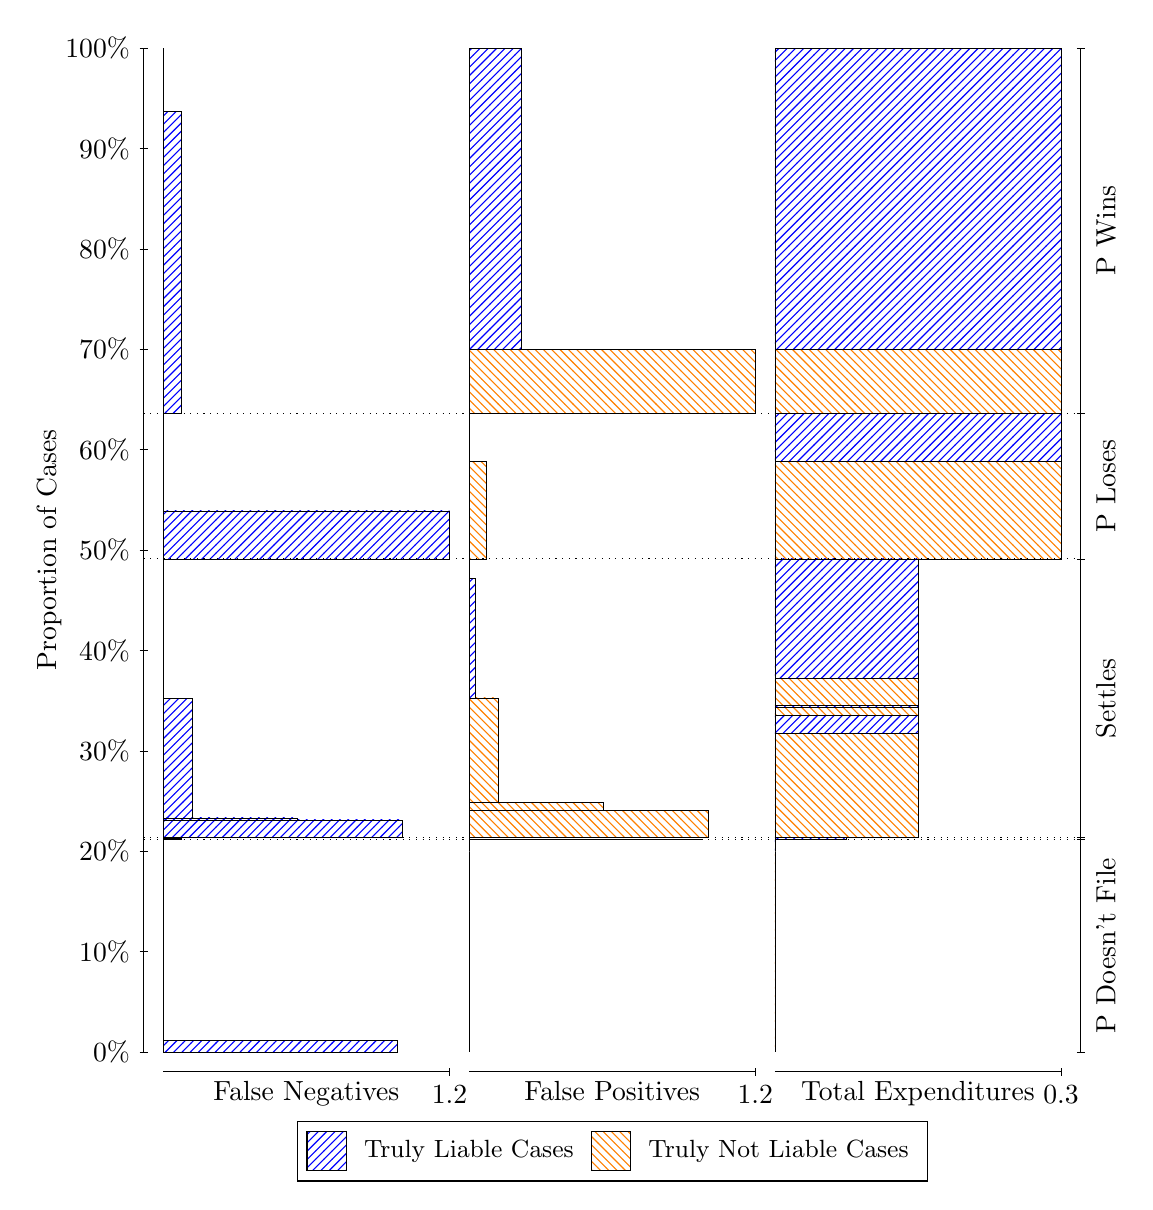
\begin{tikzpicture}
\draw[black, very thin] (1.5,1.75) -- (1.5,14.5);
\node[rotate=90, anchor=center] at (0.3, 8.125) {Proportion of Cases};
\draw[black, very thin] (1.45,1.75) -- (1.55,1.75);
\node[anchor=east] at (1.45, 1.75) {0\%};
\draw[black, very thin] (1.45,3.025) -- (1.55,3.025);
\node[anchor=east] at (1.45, 3.025) {10\%};
\draw[black, very thin] (1.45,4.3) -- (1.55,4.3);
\node[anchor=east] at (1.45, 4.3) {20\%};
\draw[black, very thin] (1.45,5.575) -- (1.55,5.575);
\node[anchor=east] at (1.45, 5.575) {30\%};
\draw[black, very thin] (1.45,6.85) -- (1.55,6.85);
\node[anchor=east] at (1.45, 6.85) {40\%};
\draw[black, very thin] (1.45,8.125) -- (1.55,8.125);
\node[anchor=east] at (1.45, 8.125) {50\%};
\draw[black, very thin] (1.45,9.4) -- (1.55,9.4);
\node[anchor=east] at (1.45, 9.4) {60\%};
\draw[black, very thin] (1.45,10.675) -- (1.55,10.675);
\node[anchor=east] at (1.45, 10.675) {70\%};
\draw[black, very thin] (1.45,11.95) -- (1.55,11.95);
\node[anchor=east] at (1.45, 11.95) {80\%};
\draw[black, very thin] (1.45,13.225) -- (1.55,13.225);
\node[anchor=east] at (1.45, 13.225) {90\%};
\draw[black, very thin] (1.45,14.5) -- (1.55,14.5);
\node[anchor=east] at (1.45, 14.5) {100\%};

\draw[black, very thin] (13.4,1.75) -- (13.4,14.5);
\draw[black, very thin] (13.35,1.75) -- (13.45,1.75);
\node[anchor=west] at (13.35, 1.75) {};
\draw[black, very thin] (13.35,4.4466) -- (13.45,4.4466);
\node[anchor=west] at (13.35, 4.4466) {};
\draw[black, very thin] (13.35,4.4738) -- (13.45,4.4738);
\node[anchor=west] at (13.35, 4.4738) {};
\draw[black, very thin] (13.35,8.0128) -- (13.45,8.0128);
\node[anchor=west] at (13.35, 8.0128) {};
\draw[black, very thin] (13.35,9.8618) -- (13.45,9.8618);
\node[anchor=west] at (13.35, 9.8618) {};
\draw[black, very thin] (13.35,14.5) -- (13.45,14.5);
\node[anchor=west] at (13.35, 14.5) {};

\draw[black, very thin, pattern color=blue, pattern=north east lines] (1.75,1.75) rectangle (4.716,1.898);
\draw[black, very thin, pattern color=orange, pattern=north west lines] (1.75,1.898) rectangle (1.75,4.4466);
\draw[black, very thin, pattern color=blue, pattern=north east lines] (1.75,4.4466) rectangle (1.9724,4.4682);
\draw[black, very thin, pattern color=orange, pattern=north west lines] (1.75,4.4682) rectangle (1.75,4.4738);
\draw[black, very thin, pattern color=blue, pattern=north east lines] (1.75,4.4738) rectangle (4.7901,4.6989);
\draw[black, very thin, pattern color=blue, pattern=north east lines] (1.75,4.6989) rectangle (3.4554,4.723);
\draw[black, very thin, pattern color=blue, pattern=north east lines] (1.75,4.723) rectangle (2.1207,6.2407);
\draw[black, very thin, pattern color=orange, pattern=north west lines] (1.75,6.2407) rectangle (1.75,8.0128);
\draw[black, very thin, pattern color=blue, pattern=north east lines] (1.75,8.0128) rectangle (5.3833,8.6206);
\draw[black, very thin, pattern color=orange, pattern=north west lines] (1.75,8.6206) rectangle (1.75,9.8618);
\draw[black, very thin, pattern color=blue, pattern=north east lines] (1.75,9.8618) rectangle (1.9724,13.692);
\draw[black, very thin, pattern color=orange, pattern=north west lines] (1.75,13.692) rectangle (1.75,14.5);
\draw[black, very thin, pattern color=orange, pattern=north west lines] (5.6333,1.75) rectangle (5.6333,4.2986);
\draw[black, very thin, pattern color=blue, pattern=north east lines] (5.6333,4.2986) rectangle (5.6333,4.4466);
\draw[black, very thin, pattern color=orange, pattern=north west lines] (5.6333,4.4466) rectangle (8.5993,4.4522);
\draw[black, very thin, pattern color=blue, pattern=north east lines] (5.6333,4.4522) rectangle (5.6333,4.4738);
\draw[black, very thin, pattern color=orange, pattern=north west lines] (5.6333,4.4738) rectangle (8.6735,4.8166);
\draw[black, very thin, pattern color=orange, pattern=north west lines] (5.6333,4.8166) rectangle (7.3388,4.9206);
\draw[black, very thin, pattern color=orange, pattern=north west lines] (5.6333,4.9206) rectangle (6.0041,6.2459);
\draw[black, very thin, pattern color=blue, pattern=north east lines] (5.6333,6.2459) rectangle (5.7075,7.7636);
\draw[black, very thin, pattern color=blue, pattern=north east lines] (5.6333,7.7636) rectangle (5.6333,8.0128);
\draw[black, very thin, pattern color=orange, pattern=north west lines] (5.6333,8.0128) rectangle (5.8558,9.2539);
\draw[black, very thin, pattern color=blue, pattern=north east lines] (5.6333,9.2539) rectangle (5.6333,9.8618);
\draw[black, very thin, pattern color=orange, pattern=north west lines] (5.6333,9.8618) rectangle (9.2667,10.669);
\draw[black, very thin, pattern color=blue, pattern=north east lines] (5.6333,10.669) rectangle (6.3007,14.5);
\draw[black, very thin, pattern color=orange, pattern=north west lines] (9.5167,1.75) rectangle (9.5167,4.2986);
\draw[black, very thin, pattern color=blue, pattern=north east lines] (9.5167,4.2986) rectangle (9.5167,4.4466);
\draw[black, very thin, pattern color=orange, pattern=north west lines] (9.5167,4.4466) rectangle (10.425,4.4522);
\draw[black, very thin, pattern color=blue, pattern=north east lines] (9.5167,4.4522) rectangle (10.425,4.4738);
\draw[black, very thin, pattern color=orange, pattern=north west lines] (9.5167,4.4738) rectangle (11.333,5.7991);
\draw[black, very thin, pattern color=blue, pattern=north east lines] (9.5167,5.7991) rectangle (11.333,6.0242);
\draw[black, very thin, pattern color=orange, pattern=north west lines] (9.5167,6.0242) rectangle (11.333,6.1283);
\draw[black, very thin, pattern color=blue, pattern=north east lines] (9.5167,6.1283) rectangle (11.333,6.1524);
\draw[black, very thin, pattern color=orange, pattern=north west lines] (9.5167,6.1524) rectangle (11.333,6.4951);
\draw[black, very thin, pattern color=blue, pattern=north east lines] (9.5167,6.4951) rectangle (11.333,8.0128);
\draw[black, very thin, pattern color=orange, pattern=north west lines] (9.5167,8.0128) rectangle (13.15,9.2539);
\draw[black, very thin, pattern color=blue, pattern=north east lines] (9.5167,9.2539) rectangle (13.15,9.8618);
\draw[black, very thin, pattern color=orange, pattern=north west lines] (9.5167,9.8618) rectangle (13.15,10.669);
\draw[black, very thin, pattern color=blue, pattern=north east lines] (9.5167,10.669) rectangle (13.15,14.5);
\draw[black, dotted] (1.5,4.4466) -- (13.4,4.4466);
\draw[black, dotted] (1.5,4.4738) -- (13.4,4.4738);
\draw[black, dotted] (1.5,8.0128) -- (13.4,8.0128);
\draw[black, dotted] (1.5,9.8618) -- (13.4,9.8618);
\draw[black, very thin] (1.75,1.5) -- (5.3833,1.5);
\node[anchor=north] at (3.5667, 1.5) {False Negatives};
\draw[black, very thin] (5.3833,1.45) -- (5.3833,1.55);
\node[anchor=north] at (5.3833, 1.45) {1.2};

\draw[black, very thin] (5.6333,1.5) -- (9.2667,1.5);
\node[anchor=north] at (7.45, 1.5) {False Positives};
\draw[black, very thin] (9.2667,1.45) -- (9.2667,1.55);
\node[anchor=north] at (9.2667, 1.45) {1.2};

\draw[black, very thin] (9.5167,1.5) -- (13.15,1.5);
\node[anchor=north] at (11.333, 1.5) {Total Expenditures};
\draw[black, very thin] (13.15,1.45) -- (13.15,1.55);
\node[anchor=north] at (13.15, 1.45) {0.3};

\node[black, centered, rotate=90] at (13.72, 3.0983) {P Doesn't File};

\node[black, centered, rotate=90] at (13.72, 6.2433) {Settles};
\node[black, centered, rotate=90] at (13.72, 8.9373) {P Loses};
\node[black, centered, rotate=90] at (13.72, 12.181) {P Wins};

\draw (7.449999999999999,1.5) node[draw=none] (baseCoordinate) {};
\begin{scope}[align=center]
        \matrix[scale=0.5, draw=black, below=0.5cm of baseCoordinate, nodes={draw}, column sep=0.1cm]{
            \node[rectangle, draw, minimum width=0.5cm, minimum height=0.5cm, pattern=north east lines, pattern color=blue] {}; &
            \node[draw=none, font=\small] (B) {Truly Liable Cases}; &
            \node[rectangle, draw, minimum width=0.5cm, minimum height=0.5cm, pattern=north west lines, pattern color=orange] {}; &
            \node[draw=none, font=\small] (B) {Truly Not Liable Cases}; \\
            };
\end{scope}

\end{tikzpicture}
\end{document}